\documentclass[10pt]{article}

\usepackage[hmarginratio=1:1,top=32mm,columnsep=20pt]{geometry}                       	
\usepackage{graphicx}
\usepackage{subcaption}
\usepackage[backend=bibtex]{biblatex}
\addbibresource{references.bib}

\title{Healthcare Data Lake}

\author{
	\textsc{Kendal, Joseph}\\
	\normalsize University of Bristol\\
	\texttt{jk17246@bristol.ac.uk}
	
	\and
	
	\textsc{Sherred, Jago}\\
	\normalsize University of Bristol\\
	\texttt{j.sherred.2019@bristol.ac.uk}
	
	\and
	
	\textsc{Benson, Luke}\\
	\normalsize University of Bristol\\
	\texttt{wr19606@bristol.ac.uk}
	
	\and
	
	\textsc{Liu, Anna}\\
	\normalsize University of Bristol\\
	\texttt{gf19916@bristol.ac.uk}
	
	\and
	
	\textsc{Cismaru, Armand}\\
	\normalsize University of Bristol\\
	\texttt{fz19792@bristol.ac.uk}
}


\begin{document}

\maketitle    


\begin{abstract}

Digital healthcare provided by the NHS in England typically operates in silos. GPs have electronic systems to manage patient care which are distinct from hospital systems which are distinct from the ambulance service, 111, mental health services etc. Each data owner has a wealth of data that, if combined, would generate a more valuable resource than it does in isolation. While there are solutions to integrate this data for direct care purposes, there is no centralised solution to use this data to inform future care or service provisioning. This project is designed to explore the benefits of cloud technologies to produce a prototype secure, scalable health data storage platform that can underpin local healthcare analytics.

\end{abstract}

\section{Overview}
%TODO%

\subsection{Client}
%TODO%
\subsection{Domain}
%TODO%
\subsection{Project}
%TODO%
\subsection{Vision}

\newpage


\section{Requirements}
\subsection{Stakeholders}
\paragraph{Primary stakeholder}
Philip Harfield at Bristol, North Somerset and South Gloucestershire CCG (BNSSG). Philip Harfield is our client, and this software is being developed for him at BNSSG. BNSSG require a piece of software to store healthcare data from various sources to inform clinical and strategic decisions. This means that BNSSG is our primary stakeholder.
\paragraph{Additional stakeholders}
This software will provide services to a number of local healthcare organisations such as NHS trusts and the Healthier Together STP and such all these additional users are secondary stakeholders to this project. These organisations will need to be able to provide healthcare information to the software which will need to be able to load and store the data for future analysis.

\subsection{User stories}
\paragraph{API}
%TODO%
\subparagraph{HL7 FHIR}
%TODO%
\subparagraph{OpenAPI}
%TODO%

\paragraph{Data lake}
%TODO%
\paragraph{Data catalogue}
%TODO%
\paragraph{ETL \& console}
%TODO%

\newpage

\section{Personal Data, Privacy, Security and Ethics Management}
\subsection{GDPR}
\subsection{Security}
\subsection{Ethics}

\newpage
\section{Architecture}
\subsection{Introduction}
We propose a modular, (cloud)platform-independent solution that offers high scalability and performance at a low cost for maintenance, development and deployment. The key to achieving this is leveraging the practises of infrastructure-as-code (IaC), serverless architectures and open standards. Therefore, development expense is focused on providing the most value, security and flexibility to the user.\\

\begin{figure}[h!]
	\centering
	\begin{subfigure}{0.25\linewidth}
		
\includegraphics[width=\linewidth]{images/Terraform.png}
	\end{subfigure}
	\begin{subfigure}{0.25\linewidth}
		
\includegraphics[width=\linewidth]{images/Serverless.png}
	\end{subfigure}
	\begin{subfigure}{0.25\linewidth}
		
\includegraphics[width=\linewidth]{images/OpenAPI.png}
	\end{subfigure}
\end{figure}

\paragraph{IaC}
By building infrastructure through extensible configuration files, we make it easy to build, test, secure, update and rollback versions of architecture which can combine multiple cloud or on-premise services. Terraform is an IaC framework that supports all major cloud providers in addition to self-hosted options such as Kubernetes. This makes it a popular choice for a modern infrastructure team that seeks to avoid vendor lock-in and easily protect the security of it with robust tests and auditing.

\begin{figure}[h!]
	\centering
	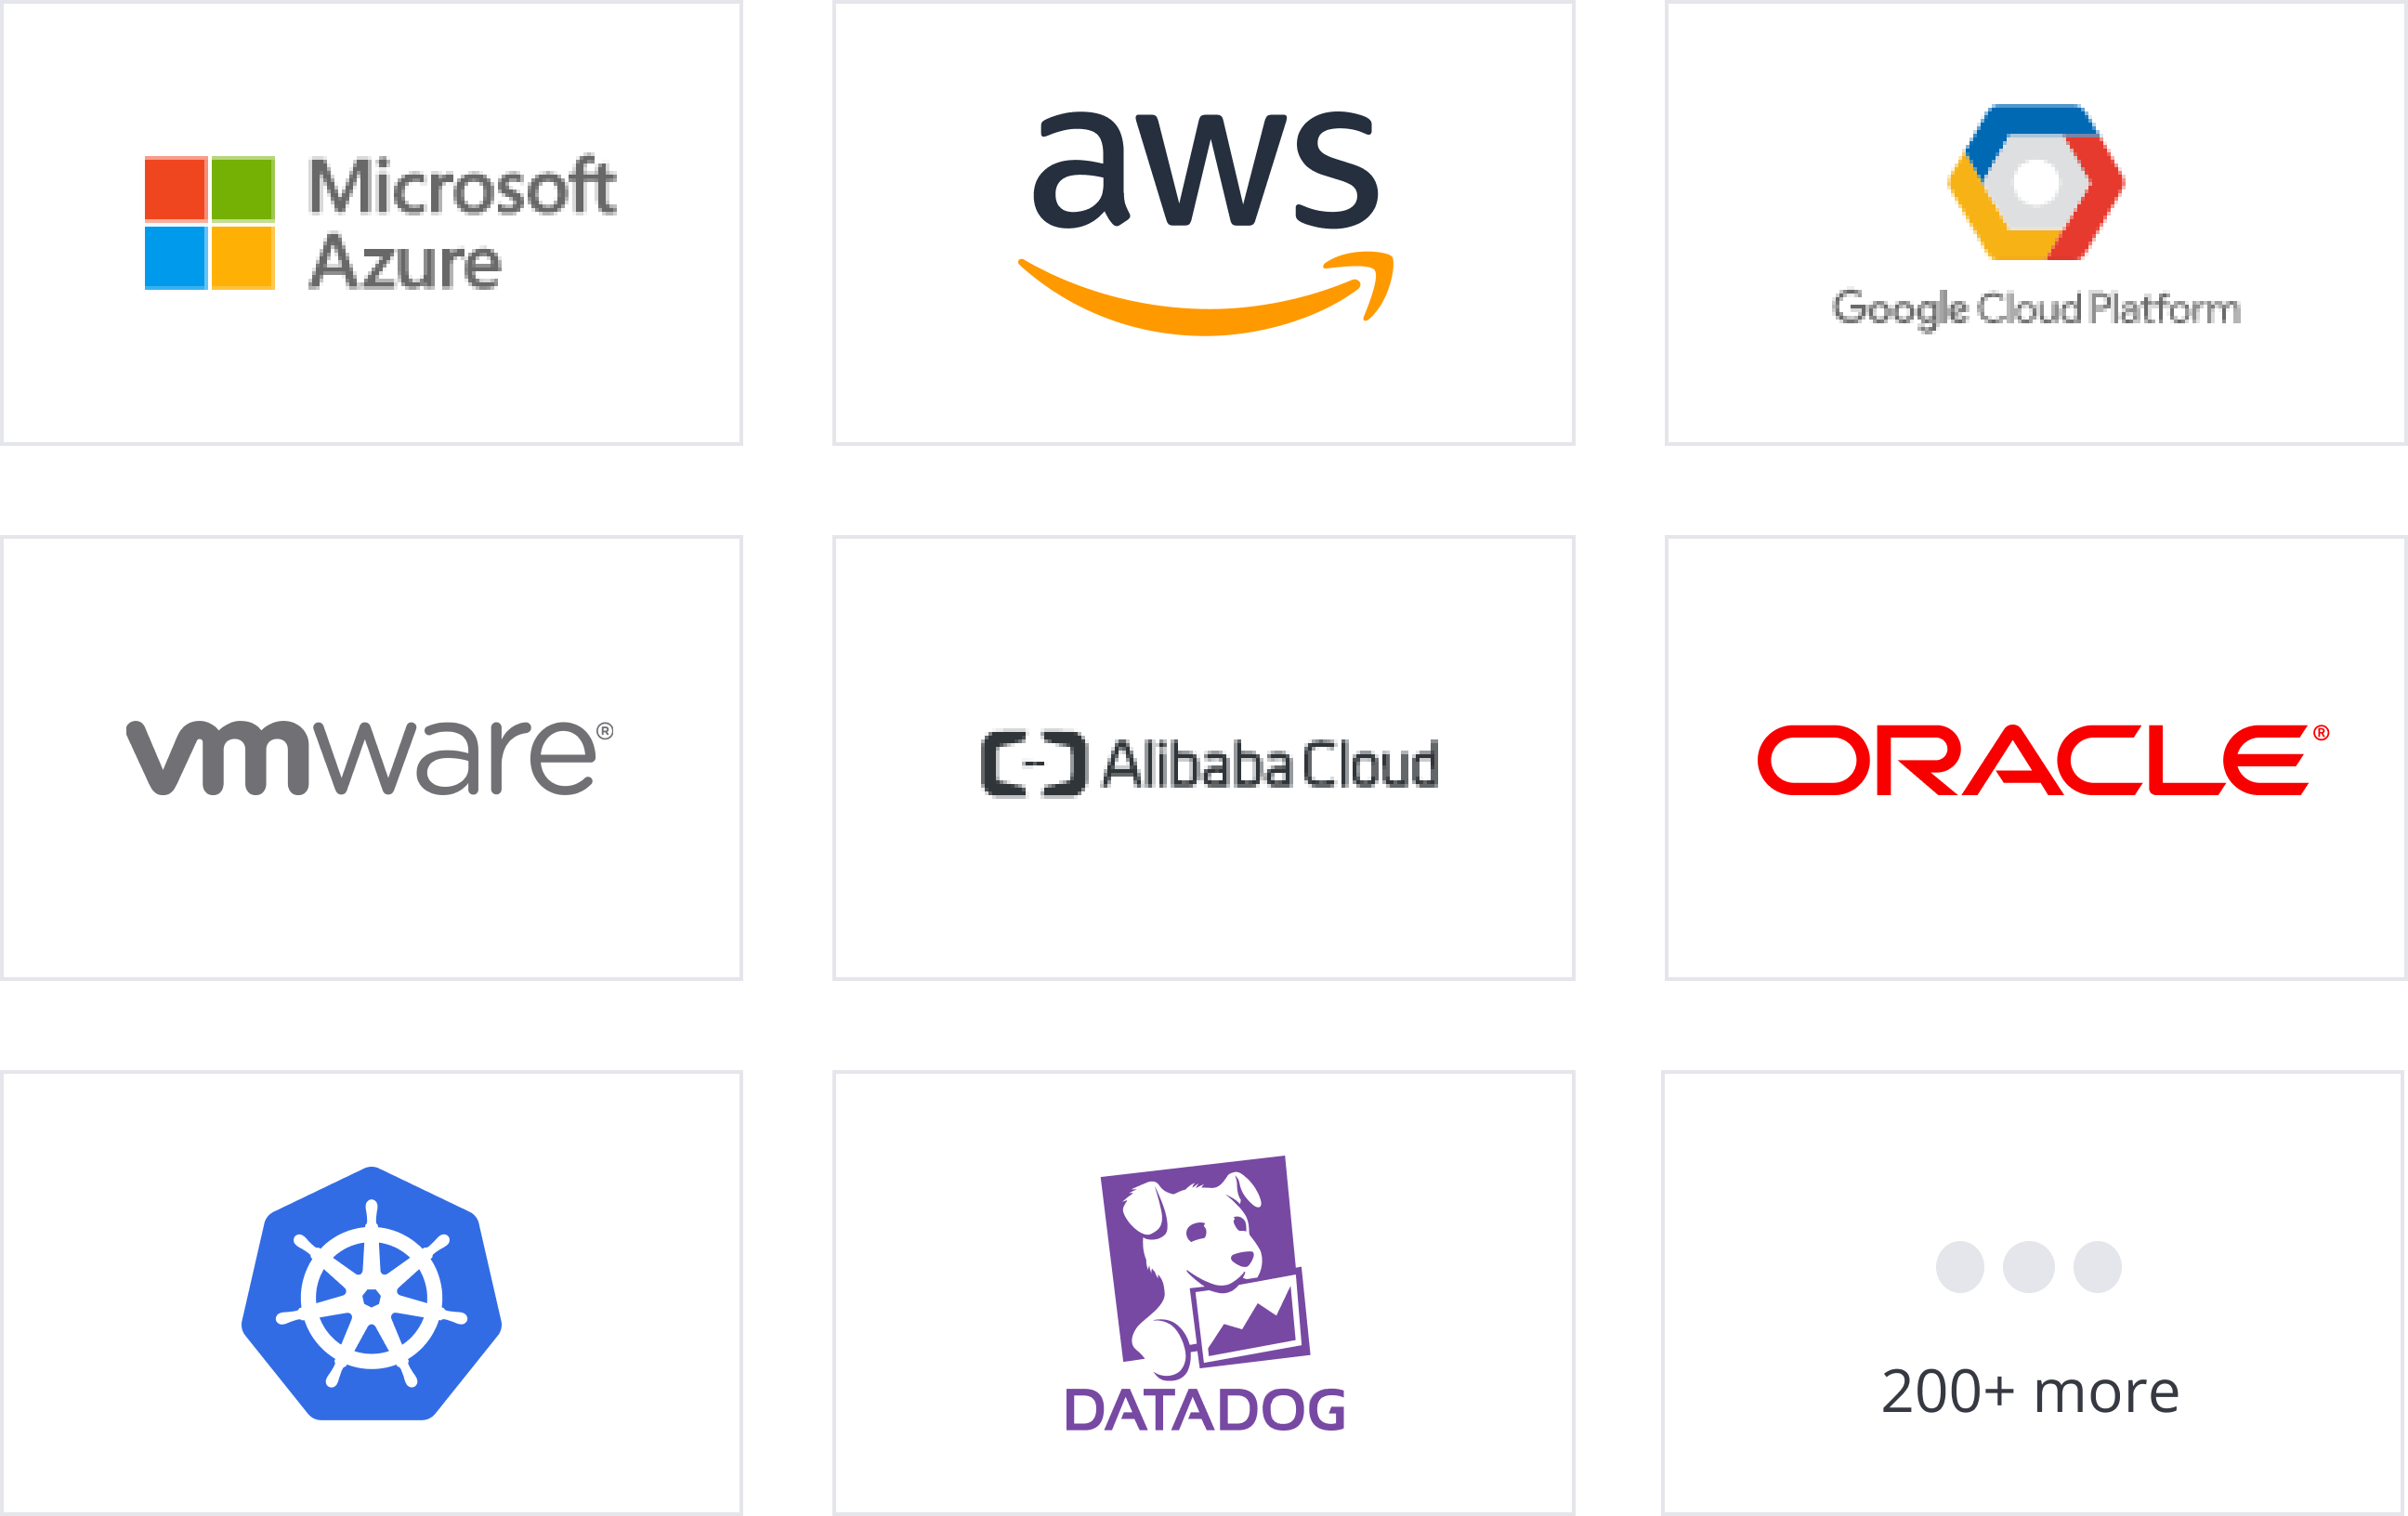
\includegraphics[width=0.65\linewidth]{images/TerraformProviders.png}	
\end{figure}

\paragraph{Serverless}
Serverless computing is a cloud computing execution model in which the cloud provider runs the server, and dynamically manages the allocation of machine resources. Pricing is based on the actual amount of resources consumed by an application, rather than on pre-purchased units of capacity \parencite{serverless}. The benefits of this approach are the huge reduction in infrastructure and development expense. Engineers can focus on shipping their microservices and have secure, scalable infrastructure taken care of for them.
\\ \\
The Serverless Framework is also an example of IaC and provides developers with the ability to develop and deploy their serverless application to different cloud providers or simply Kubernetes (using \textbf{Knative}) if they wanted to run it on-premise or avoid code exposure to a cloud native service such as AWS Lambda or Google Cloud Functions.

\paragraph{Open standards}
\subparagraph{OpenAPI}
%TODO%
\subparagraph{HL7 FHIR}
%TODO%

\subsection{Data ingestion}
\subsubsection{Microservices}
\subsubsection{Metadata cataloguing}
\subsubsection{Schema-less object store}

\subsection{Data warehousing}
\subsubsection{Federated querying}
\subsubsection{Common models}

\subsection{ETL \& data marts}
\subsubsection{Scheduling}
\subsubsection{Developers}
\subsubsection{Console}

\subsection{Secure access}
\subsubsection{Encryption}
\subsubsection{IAM}
\subsubsection{Logging}

\newpage
\section{Development Testing}
\subsection{Local environment}
\subsubsection{API development}
%TODO%
\paragraph{Serverless}
%TODO%
\paragraph{Postman}

Postman is a very popular tool used by developers that want to conveniently test and build APIs in a collaborative way.
\\ \\
As we are implementing the OpenAPI specification, Postman enables the import of Swagger files to automatically generate a Postman environment. This makes developer on-boarding much easier as versioned mock endpoints and documentation are hosted for us as part of the DevOps deployment.


\subsection{DevOps pipeline}
\subsubsection{GitHub}
\subsubsection{CircleCI}
\subsubsection{CodeDeploy}

\section{Release Testing}
\subsection{Staging}
\subsection{Production}

\newpage
\section{OO Design \& UML}

\printbibliography

\end{document}
